\documentclass[8pt,a4paper,compress]{beamer}

\usepackage{/home/siyer/lib/slides}

\usepackage{fancyvrb}

\newcommand{\mm}[1]{$#1$}
\DefineVerbatimEnvironment
{production}{Verbatim}
{fontfamily=timesroman,commandchars=\\\{\}}

\title{Parsing}
\date{}

\begin{document}
\begin{frame}
\vfill
\titlepage
\end{frame}

\begin{frame}
\frametitle{Outline}
\tableofcontents
\end{frame}

\section{Introduction}
\begin{frame}[fragile]
\pause

Once we have identified the tokens in our program, we then want to determine its syntactic structure and the process of doing so is called parsing

\pause
\bigskip

We wish to make sure the program is syntactically valid, ie, it conforms to the grammar that describes its syntax

\pause
\bigskip

As the parser parses the program it should identify syntax errors and report them and the line numbers they appear on

\pause
\bigskip

When the parser does find a syntax error, it should not just stop, but it should report the error, and gracefully recover so that it may go on looking for additional errors

\pause
\bigskip

The parser should produce some representation of the parsed program that is suitable for semantic analysis; in the \jmm compiler, we produce an abstract syntax tree (AST)
\end{frame}

\begin{frame}[fragile]
\pause

For example, given the following \jmm program

\begin{lstlisting}[language=Java]
package pass;

import java.lang.System;

public class Factorial {
    // Two methods and a field
    public static int factorial(int n) {
        if (n <= 0)
            return 1;
        else
            return n * factorial(n - 1);
    }
    
    public static void main(String[] args) {
        int x = n;
        System.out.println(x + "! = " + factorial(x));
    }

    static int n = 5;
}
\end{lstlisting}
we would like to produce an AST shown in the following slide
\end{frame}

\begin{frame}[fragile]
\pause

AST for the \lstinline{Factorial} program
\begin{center}
\visible<2->{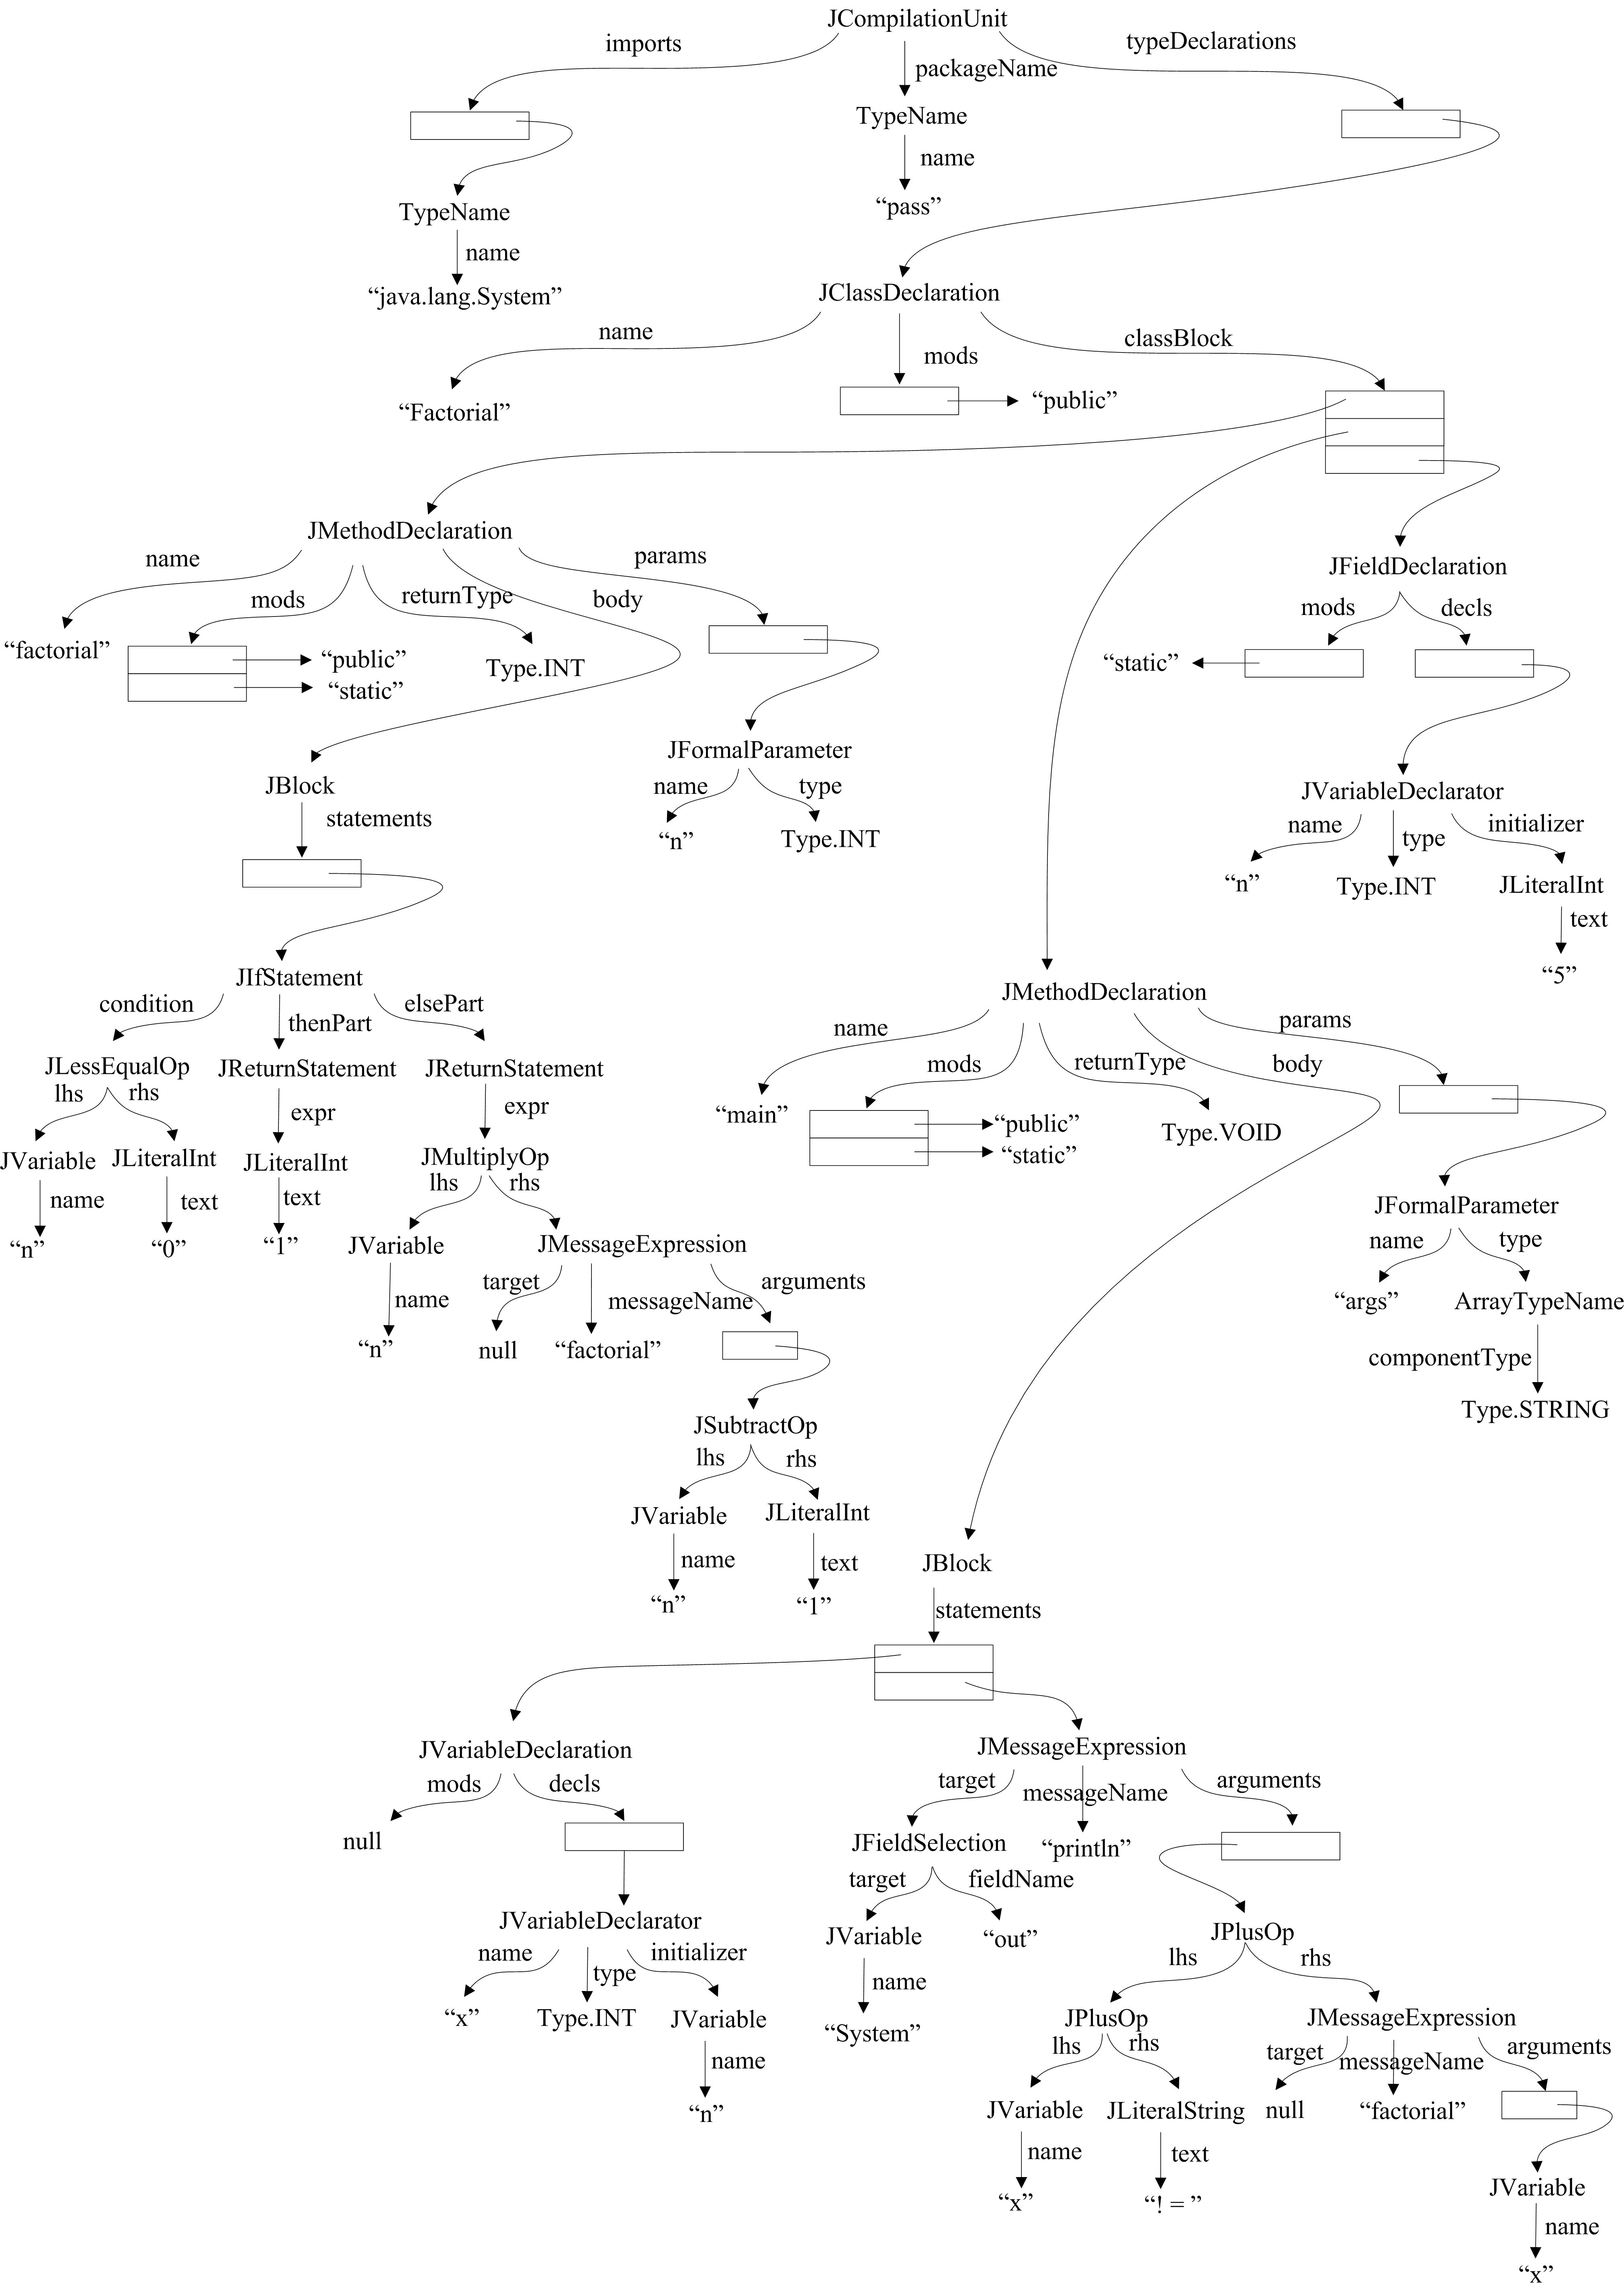
\includegraphics[scale=0.29]{{figures/figure03.01}.jpg}}
\end{center}
\end{frame}

\begin{frame}[fragile]
\pause

The nodes in the AST represent syntactic objects

\pause
\bigskip

The AST is rooted at a \lstinline{JCompilationUnit}, the syntactic object representing the program that we are compiling

\pause
\bigskip

The directed edges are labeled by the names of the fields they represent; for example, \lstinline{JCompilationUnit} has a package name, a list (an \lstinline{ArrayList}) of imported types, and a list (an \lstinline{ArrayList}) of class declarations

\pause
\bigskip

We are interested in a tree representation for our program because it is easier to analyze and decorate (with type information) a tree than it is to do the same with text

\pause
\bigskip

The AST makes the syntax implicit in the program text, explicit, which is essentially the purpose of parsing
\end{frame}

\section{Context-free Grammars and Languages}
\begin{frame}[fragile]
\pause

The grammars that we use to describe programming languages are inherently recursive and are best described by what we call context-free grammars

\pause
\bigskip

The notation for describing programming language is called Backus-Naur Form (BNF)

\pause
\bigskip

For example, the context-free rule

\begin{production}
\mm{S} ::=  \lstinline{if} \lstinline{(}\mm{E}\lstinline{)} \mm{S}
\end{production}

\noindent says that, if \mm{E} is an expression and \mm{S} is a statement, then 

\begin{production}
\lstinline{if} \lstinline{(}\mm{E}\lstinline{)} \mm{S}
\end{production}

\noindent is also a statement

\pause
\bigskip

There are abbreviations possible in the notation; for example, we can write

\begin{production}
\mm{S} ::= \lstinline{if} \lstinline{(}\mm{E}\lstinline{)} \mm{S}
      \mm{|} \lstinline{if} \lstinline{(}\mm{E}\lstinline{)} \mm{S} \lstinline{else} \mm{S}
\end{production}

\noindent as shorthand for

\begin{production}
\mm{S} ::= \lstinline{if} \lstinline{(}\mm{E}\lstinline{)} \mm{S}
\mm{S} ::= \lstinline{if} \lstinline{(}\mm{E}\lstinline{)} \mm{S} \lstinline{else} \mm{S}
\end{production}
\end{frame}

\begin{frame}[fragile]
\pause

Square brackets indicate that a phrase is optional; for example, the two rules from above can be written as

\begin{production}
\mm{S} ::=  \lstinline{if} \lstinline{(}\mm{E}\lstinline{)} \mm{S} [\lstinline{else} \mm{S}]
\end{production}

\pause

Curly braces denote the Kleene closure, indicating that the phrase may appear zero or more times; for example

\begin{production}
\mm{E} ::= \mm{T} \{\lstinline{\+} \mm{T}\}
\end{production}

\noindent says that an expression $E$ may be written as a term $T$, followed by zero or more  occurrences of \lstinline{+} followed by a term $T$, such as

\begin{production}
\mm{T} \lstinline{+} \mm{T} \lstinline{+} \mm{T} \mm{\dots}
\end{production}

\pause

One may use the alternation sign $|$ inside right-hand-sides, using parentheses for grouping; for example

\begin{production}
\mm{E} ::= \mm{T} \{(\lstinline{\+} \mm{|} \lstinline{\-}) \mm{T}\}
\end{production}

\noindent means that the additive operator may be either \lstinline{+} or \lstinline{-}, such as

\begin{production}
\mm{T} \lstinline{+} \mm{T} \lstinline{\-} \mm{T} \lstinline{+} \mm{T}
\end{production}

\pause

BNF allows us to describe such syntax as that for a \jmm compilation unit

\begin{production}
compilationUnit ::= [\lstinline{package} qualifiedIdentifier \lstinline{;}]
                           \{\lstinline{import}  qualifiedIdentifier \lstinline{;}\}
                           \{typeDeclaration\} \lstinline{EOF}
\end{production}
\end{frame}

\section{Top-down Deterministic Parsing}
\begin{frame}[fragile]
\pause

\end{frame}

\section{Bottom-up Deterministic Parsing}
\begin{frame}[fragile]
\pause

\end{frame}

\section{Parser Generation Using JavaCC}
\begin{frame}[fragile]
\pause

\end{frame}
\end{document}
